% !TEX program = xelatex

\documentclass[aspectratio=169]{beamer}

\usepackage{xltxtra} 
\usetheme{focus}
\XeTeXlinebreaklocale "th_TH"
\usepackage{fontspec}
\defaultfontfeatures{Mapping=tex-text,Scale=MatchLowercase}
% \setsansfont{Gillius ADF No2}
% \setmonofont{Tlwg Typist}
\usepackage{listings}
\usepackage{color}
\usepackage{amsmath}
\usepackage{smartdiagram}
\usepackage{graphicx}
\usepackage{tikz}
\usepackage{multicol}

\lstdefinestyle{codeblock}{
    breakatwhitespace=false,         
    breaklines=true,                 
    captionpos=b,                    
    keepspaces=true,              
    showspaces=false,                
    showstringspaces=true,
    showtabs=false,                  
    tabsize=4
}

\lstset{style=codeblock}

\title{First Step to Practical Machine Learning}
\subtitle{Knowledge Sharing for CPE/SKE students}
\author{Sirakorn Lamyai}
\institute{Student, Kasetsart U.}
\date{October 30, 2018}
\begin{document}

\begin{frame}
	\titlepage
\end{frame}

\begin{frame}
	\frametitle{Acknowledgements}
	Resources on this slides are mainly adapted and rearranged from
	\begin{itemize}
		\item \href{https://docs.google.com/presentation/d/1oGIyzoMHT3-TTS23NPL-qzh0EAXb6kyK0S_1n5MjmgQ/edit\#slide=id.p}{W. Jitkrittum: Machine Learning Fundamentals I}
		\item \href{http://krikamol.org/tutorial/slides/vistec-talk-16-March-2018.pdf}{K. Muandet: Machine Learning Fundamentals II}
		\item \href{}{Google's Machine Learning Crash Course}
	\end{itemize}
\end{frame}

\begin{frame}
	\frametitle{Before we start...}
	Make sure these are installed on your computer.\\

	\begin{itemize}
		\item Python 3.6
		\item NumPy, Scipy, Matplotlib, Scikit-learn, MLxtend:\\
			  Run \texttt{pip install numpy scipy matplotlib sklearn mlxtend}
		\item MNIST loader\\
			  \texttt{pip install git+https://github.com/datapythonista/mnist.git}
	\end{itemize}
\end{frame}

\begin{frame}
	\frametitle{Outline}
	\begin{multicols}{2}
		\tableofcontents
	\end{multicols}
\end{frame}

\section{Introduction to Machine Learning}

\subsection{What is Machine Learning?}

\begin{frame}
	\frametitle{What is Machine Learning?}
	\pause
	\begin{figure}
		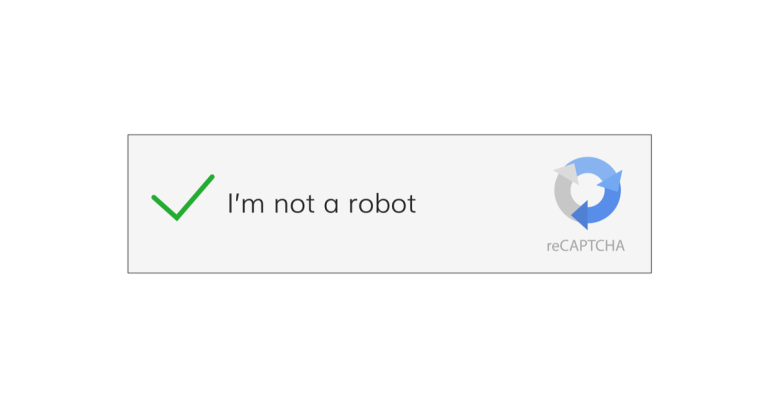
\includegraphics[scale=0.4]{imgs/recaptcha.png}
	\end{figure}
	\begin{itemize}
		\pause
		\item This is Recaptcha.
		      \begin{itemize}
			      \pause
			      \item Recaptcha helps stop millions of spam a day.
			            \pause
			      \item In some old days, we have to type Captcha texts to distinguish ourself from bots.
			            \pause
			      \item How is it possible that with a single click, an automated system can distinguish bots from humans?
		      \end{itemize}
	\end{itemize}
\end{frame}

\begin{frame}
	\frametitle{Machine Learning}
	\begin{center}
		Machine Learning \\
		\onslide<2-> \huge = Improves performance on a specific task.
	\end{center}
\end{frame}

\section{Machine Learning Problems}

\begin{frame}
	\frametitle{Types of Machine Learning problems}
	\begin{enumerate}
		\item<2-> Supervised learning
		\item<3-> Unsupervised learning
		\item<4-> Reinforcement learning
	\end{enumerate}
\end{frame}

\subsection{Supervised learning}

\begin{frame}
	\frametitle{Supervised learning}
	\begin{columns}
		\column{0.5\textwidth}
		\begin{figure}
			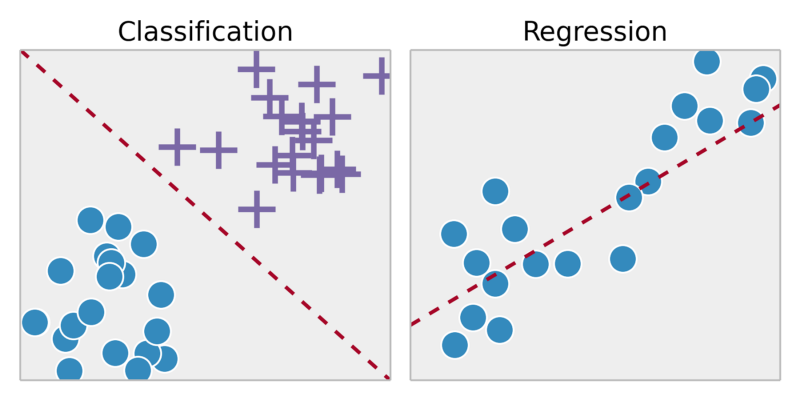
\includegraphics[width=1.0\textwidth]{imgs/supervised_learning.png}
		\end{figure}
		\column{0.5\textwidth}
		\begin{itemize}
			\item<2-> Given a \textbf{training set} for the data, find a \textbf{model} to \textbf{generalise} well to \textbf{unseen} data.
			\item<3-> Two main supervised learning problems
			      \begin{itemize}
				      \item<4-> Classification: On the discrete data
				      \item<5-> Regression: On the continuous data
			      \end{itemize}
			\item<6-> Example problems: Spam E-mail detection, Facial recognition
		\end{itemize}
	\end{columns}
\end{frame}

\subsection{Unsupervised learning}

\begin{frame}
	\frametitle{Unsupervised learning}
	\begin{columns}
		\column{0.5\textwidth}
		\begin{figure}
			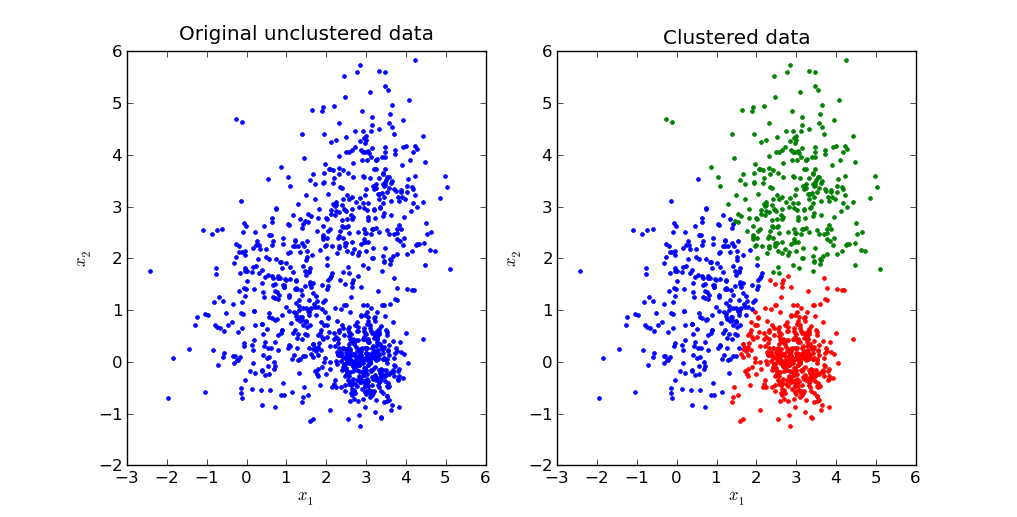
\includegraphics[width=1.0\textwidth]{imgs/kmeans.png}
		\end{figure}
		\column{0.5\textwidth}
		\begin{itemize}
			\item<2-> Discover \textbf{hidden} structure in \textbf{non-labelled} data.
			\item<3-> Example: Clustering, Generative models
		\end{itemize}
	\end{columns}
\end{frame}

\subsection{Reinforcement learning}

\begin{frame}
	\frametitle{Reinforcement learning}
	\begin{figure}
		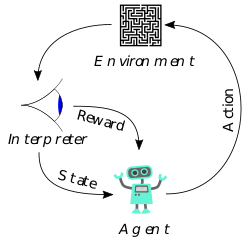
\includegraphics[scale=.7]{imgs/reinforcement_learning.png}
	\end{figure}
\end{frame}


\section{Model}

\begin{frame}
	\frametitle{Model}
	\begin{itemize}
		\item<2-> A result of the combination between...
		      \begin{itemize}
			      \item<3-> a \textbf{method} to recognise the data, and
			      \item<4-> \textbf{sample datas} for such the method
		      \end{itemize}
	\end{itemize}
	\begin{columns}
		\column<5->{0.5\textwidth}
		\begin{figure}
			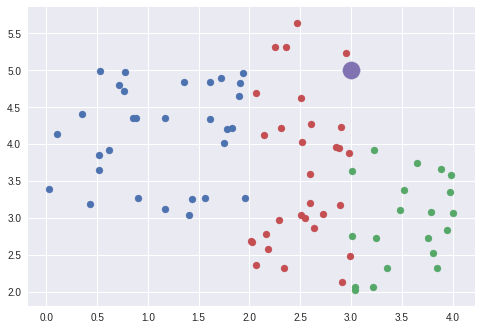
\includegraphics[scale=.3]{imgs/simple_knn.png}
		\end{figure}
		\column<6->{0.5\textwidth}
		Determine which group should the purple dot be in (red/green/blue) by \textbf{checking the colour of its nearest dot.}
	\end{columns}
	\begin{columns}
		\column{0.5\textwidth}
		\begin{center}
			\onslide<5-> \Large Data
		\end{center}
		\column{0.5\textwidth}
		\begin{center}
			\onslide<6-> \Large Method
		\end{center}
	\end{columns}
\end{frame}

\subsection{The Goal of Machine Learning}

\begin{frame}
	\frametitle{The Goal of Machine Learning}
	\begin{center}
		\Huge Generalise
	\end{center}
	\begin{itemize}
		\item We wants our model to know how does the \textbf{data pattern} looks like
		\item Our model should not "adhere" to one set of data, but instead knows the pattern of all the data.
		\item Therefore, we want our model to \textbf{generalise} over any set of data, given the small portion of data that we used to teach the model.
	\end{itemize}
\end{frame}

\begin{frame}
	\frametitle{Beginning with our first model}
	\begin{itemize}
		\item<2-> We're going to write our \textbf{first own} machine learning algorithm called \textbf{$k$-Nearest Neighbour} ($k$-NN)
		      \begin{itemize}
			      \item<3-> $k$-NN is known to be very simple, with its concept as
		      \end{itemize}
	\end{itemize}
	\onslide<4->
	\begin{block}{$k$-NN algorithm}
		To classify label of a data point, get $k$ nearest data points to the data point, and select the major label among those data points.
	\end{block}
\end{frame}

\section{Machine Learning Process}

\subsection{Evaluating Machine Learning Performance}

\begin{frame}
	\frametitle{Choosing the parameter for $k$-NN algorithm}
	\onslide<2-> What is the bad way to choose $k$?
	\begin{itemize}
		\item<3-> What if we choose $k$ = \# of all points?
		      \begin{itemize}
			      \item<4-> What will happen if our dataset's got 3 labels of A, B, C with 10, 20, and 30 data points of each?
			      \item<5-> Answer: Our model will always answer the labels with the highest data point count.
		      \end{itemize}
		\item<6-> What if we choose $k$ = 1?
		      \begin{itemize}
			      \item<7-> Let's try!
		      \end{itemize}
	\end{itemize}
\end{frame}

\begin{frame}
	\frametitle{Training Error}
	\begin{figure}
		\begin{tikzpicture}
			\draw [black] (0, 0) rectangle (10, 1) node[pos=.5] {Training data};
			\draw [->, red] (2.5, 0) -- (2.5, -1) node[pos=.5] {Train};
			\draw [black, thick] (0, -2) rectangle (5, -1) node[pos=.5] {Model};
			\draw [->, violet] (7.5, 0) -- (7.5, -1.5) -- (5, -1.5) node[pos=0] {Evaluate error};
		\end{tikzpicture}
	\end{figure}
	\begin{columns}[t]
		\column{0.5\textwidth}
		\begin{block}{Loss function}
			$$L(y, \hat{y}) =
				\begin{cases}
					0 & y = \hat{y}    \\
					1 & y \neq \hat{y}
				\end{cases}
			$$
		\end{block}
		\column{0.5\textwidth}
		\begin{block}{Error}
			$$\sigma = \frac{1}{N}\sum_{i=0}^{N}L(y_i, \hat{y}_i)$$
		\end{block}
	\end{columns}
\end{frame}

\begin{frame}
	\frametitle{What went wrong with our intuition?}
	\begin{itemize}
		\item Evaluating error with a data points that our model had already seen is bad.
		\item Why? Because our model already knows the answer to that data point! It could just simply answer by looking at the "answer key"
		\item So how should we evaluate our model?
	\end{itemize}
\end{frame}

\begin{frame}
	\frametitle{Training and Testing set}
	\begin{figure}
		\begin{tikzpicture}
			\draw [black] (0, 0) rectangle (7, 1) node[pos=.5] {Training data};
			\draw [blue] (7.5, 0) rectangle (10, 1) node[pos=.5] {Testing data};
			\draw [->, red] (2.5, 0) -- (2.5, -1) node[pos=.5] {Train};
			\draw [black, thick] (0, -2) rectangle (5, -1) node[pos=.5] {Model};
			\draw [->, violet] (8.5, 0) -- (8.5, -1.5) -- (5, -1.5) node[pos=0] {Evaluate error};
		\end{tikzpicture}
	\end{figure}
	\begin{itemize}
		\item<2-> We separate our dataset into 2 parts: the \textbf{training set} and \textbf{testing set}
			\begin{itemize}
				\item<3-> Our model sees the correct label of the training set, but not the testing set.
				\item<4-> We all know the correct label of both the training and testing set.
				\item<5-> Teach our model with the training set, see how it performs with the testing set.
			\end{itemize}
	\end{itemize}
\end{frame}

\begin{frame}
	\frametitle{Choosing the best $k$}
	What will happen if...

	\begin{itemize}
		\item our $k$ is too small?
		\item our $k$ is too large?
	\end{itemize}
\end{frame}

\begin{frame}
	\frametitle{Overfitting and underfitting}
	Which decision region is good?\\~\\
	\begin{columns}[t]
		\column{0.33\textwidth}
		\onslide<1-> 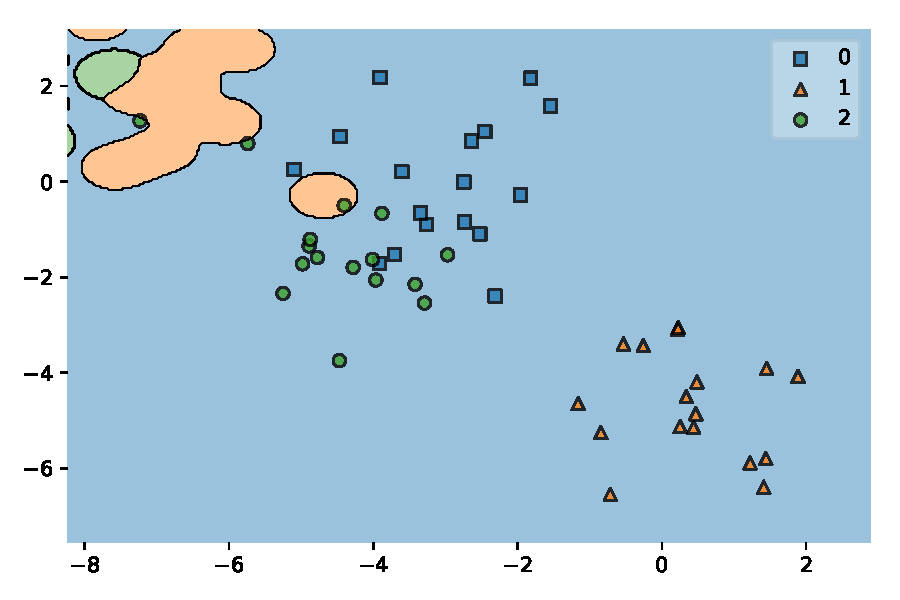
\includegraphics[width=1.0\textwidth]{imgs/underfit.pdf}
		\onslide<2-> \textbf{Underfit: } The model fails to recognise data pattern
		\column{0.33\textwidth}
		\onslide<1-> 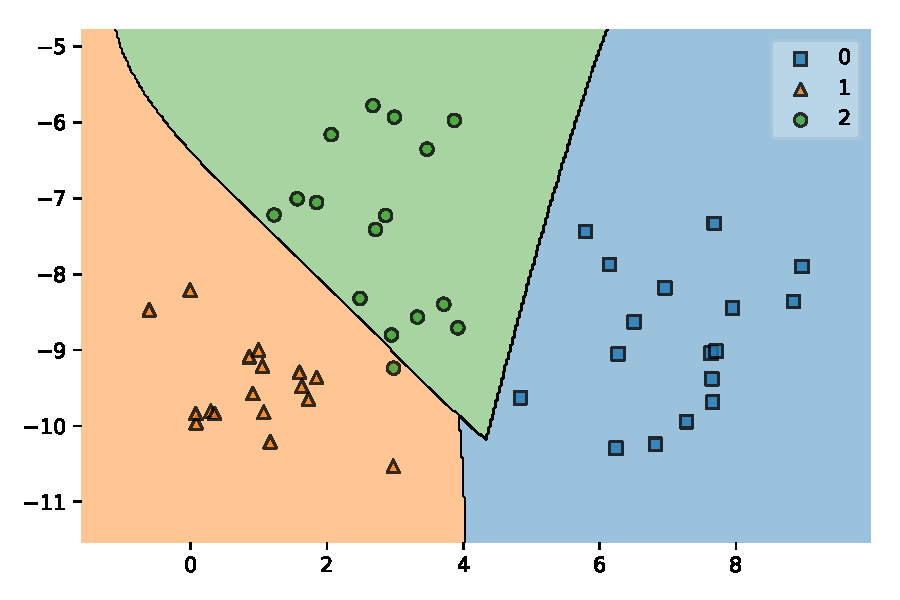
\includegraphics[width=1.0\textwidth]{imgs/good.pdf}
		\onslide<4-> \textbf{Good fit: } The model recognises data pattern \textbf{generally}
		\column{0.33\textwidth}
		\onslide<1-> 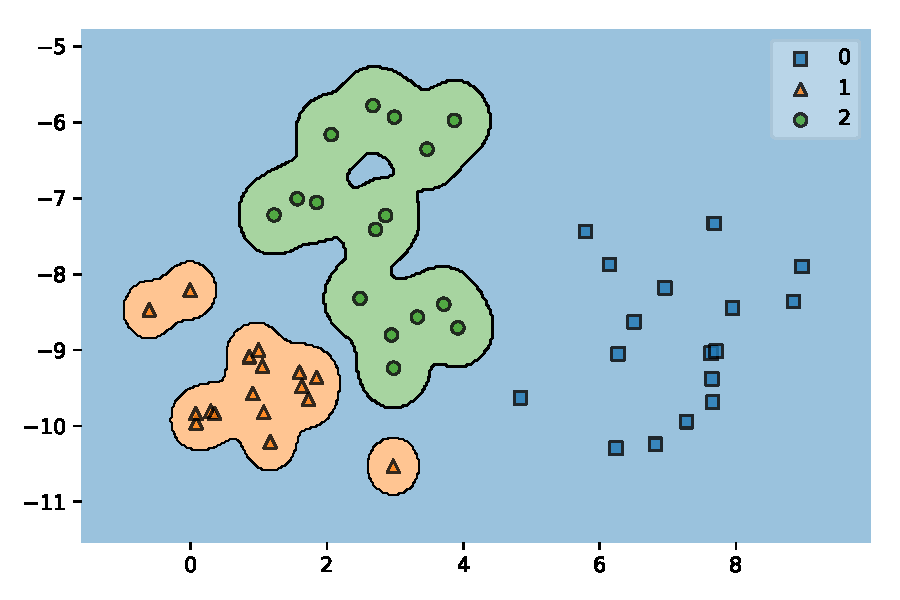
\includegraphics[width=1.0\textwidth]{imgs/overfit.pdf}
		\onslide<3-> \textbf{Overfit:} The model \textbf{remembers} data pattern instead of generalising.
	\end{columns}
\end{frame}

\begin{frame}
	\frametitle{Overfitting and underfitting}
	\begin{center}
		{\LARGE Good model must \textbf{generalise}}\\
	\end{center}
\end{frame}

\begin{frame}
	\frametitle{Parameter Optimisation}
	\begin{itemize}
		\item Actually, the key point in $k$-NN algorithm is choosing $k$ points with the least \textbf{distant}.
		\item What is \textbf{distant}?
	\end{itemize}
\end{frame}

\begin{frame}
	\frametitle{Norm for $k$-NN algorithm}
	\begin{block}{Norm}
		In linear algebra, a \textbf{norm} is a function that assigns a strictly positive length or size to each vector in a vector space - except for the zero vector, which is assigned a length of zero.
	\end{block}

	Given $\vec{x}$ as an $N$-dimension vector of $\begin{bmatrix}
			x_1 & x_2 & \hdots & x_n
		\end{bmatrix}$
	\begin{itemize}
		\item $l_1$ Norm: $\left|x\right|_1 = \sum_{i=0}^{N}\left|x_i\right|$ (Manhattan)
		\item $l_2$ Norm: $\left|x\right|_2 = \sqrt{\sum_{i=0}^{N}x_i^2}$ (Euclidian)
		\item $l_p$ Norm: $\left|x\right|_p = \left(\sum_{i=1}^n |x_i|^p\right)^{1/p}$ (Minkowski)
	\end{itemize}
\end{frame}

\section{Algorithms for Machine Learning Classification Problem}

\begin{frame}
	\frametitle{Algorithms for Machine Learning Classification Problem}
	$k$-NN is a very simple intuition for machine learning algorithms. However, there exists more algorithm that performs well to other problems.

	Example algorithms:
	\begin{itemize}
		\item Na\"{i}ve Bayes
		\item SVM
		\item Decision Tree
		\item Logistic Regression
	\end{itemize}
\end{frame}

\begin{frame}
	\frametitle{Na\"ive Bayes}
	\begin{columns}
		\column{0.4\textwidth}
		\begin{center}
			\begin{tabular}{|c | c c |}
				\hline
				  & Gender & Hair  \\ [0.5ex]
				\hline\hline
				1 & M      & Long  \\
				\hline
				2 & M      & Short \\
				\hline
				3 & F      & Long  \\
				\hline
				4 & F      & Long  \\
				\hline
				5 & F      & Short \\ [1ex]
				\hline
			\end{tabular}
		\end{center}
		\begin{block}{Bayes Theorem}
			$P(A|B) = \frac{P(A \cap B)}{P(B)} = \frac{P(B|A) \times P(A)}{P(B)}$
		\end{block}
		\column{0.6\textwidth}
		Can we \textit{guess} the gender from hair's length?
		\begin{itemize}
			\item $P(\textrm{Male}|\textrm{Long hair}) = \frac{1}{3}$
			\item $P(\textrm{Female}|\textrm{Long hair}) = \frac{2}{3}$
		\end{itemize}
		Therefore, we guess that the long-haired person is more likely to be a female.
	\end{columns}
\end{frame}

\begin{frame}
	\frametitle{Support Vector Machines (SVM)}
	\begin{columns}
		\column{0.3\textwidth}
		\onslide<1-> 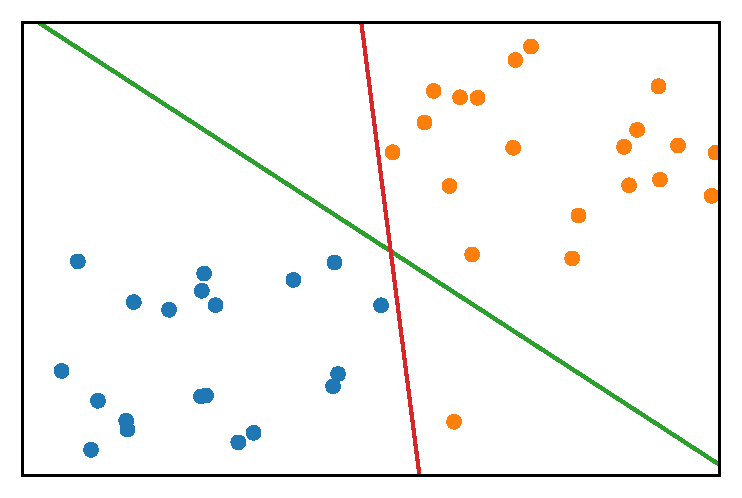
\includegraphics[width=1.0\textwidth]{imgs/svm_2.pdf}
		\column{0.3\textwidth}
		\onslide<1-> 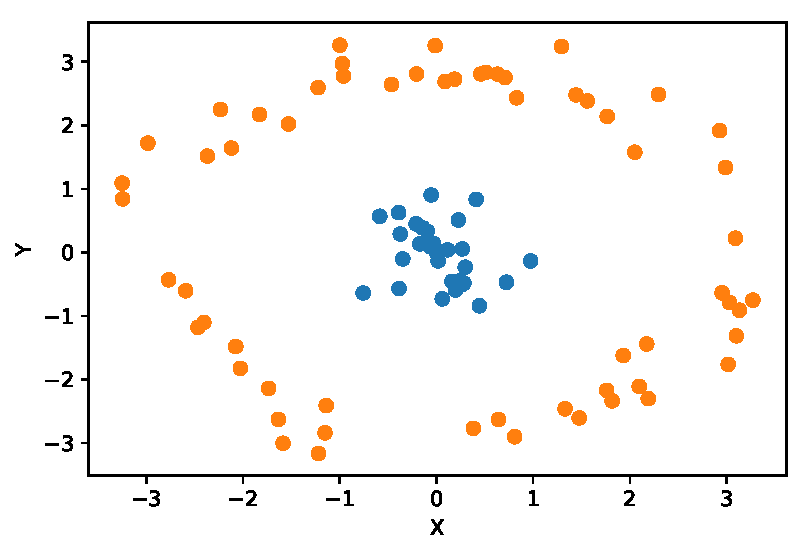
\includegraphics[width=1.0\textwidth]{imgs/svm_3.pdf}
		\onslide<1-> 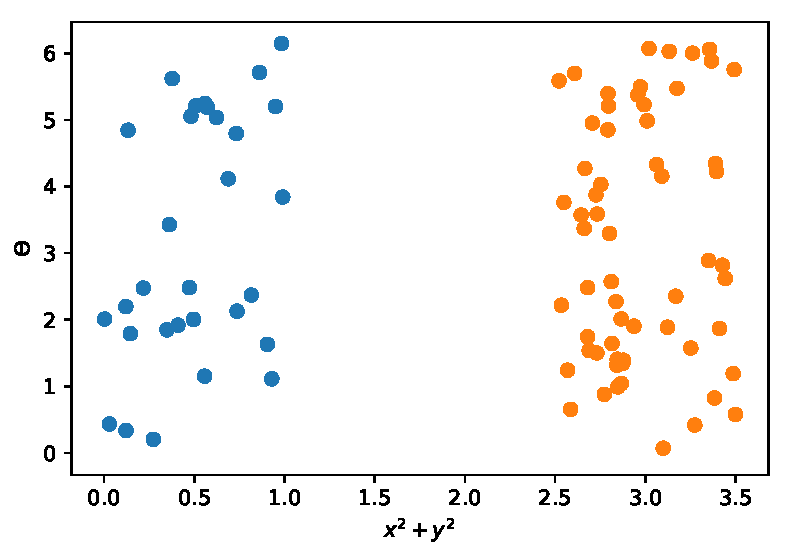
\includegraphics[width=1.0\textwidth]{imgs/svm_4.pdf}
		\column{0.4\textwidth}
		\begin{itemize}
			\item Goal: to draw a line to separate groups of data
			\item Ideal good line: maximising the distant between the line and classes of data points
			\item What if the data is not linearly separable? \textbf{Kernel tricks}
		\end{itemize}
	\end{columns}
\end{frame}

\begin{frame}
	\frametitle{Decision Tree}
	\begin{columns}
		\column{0.4\textwidth}
		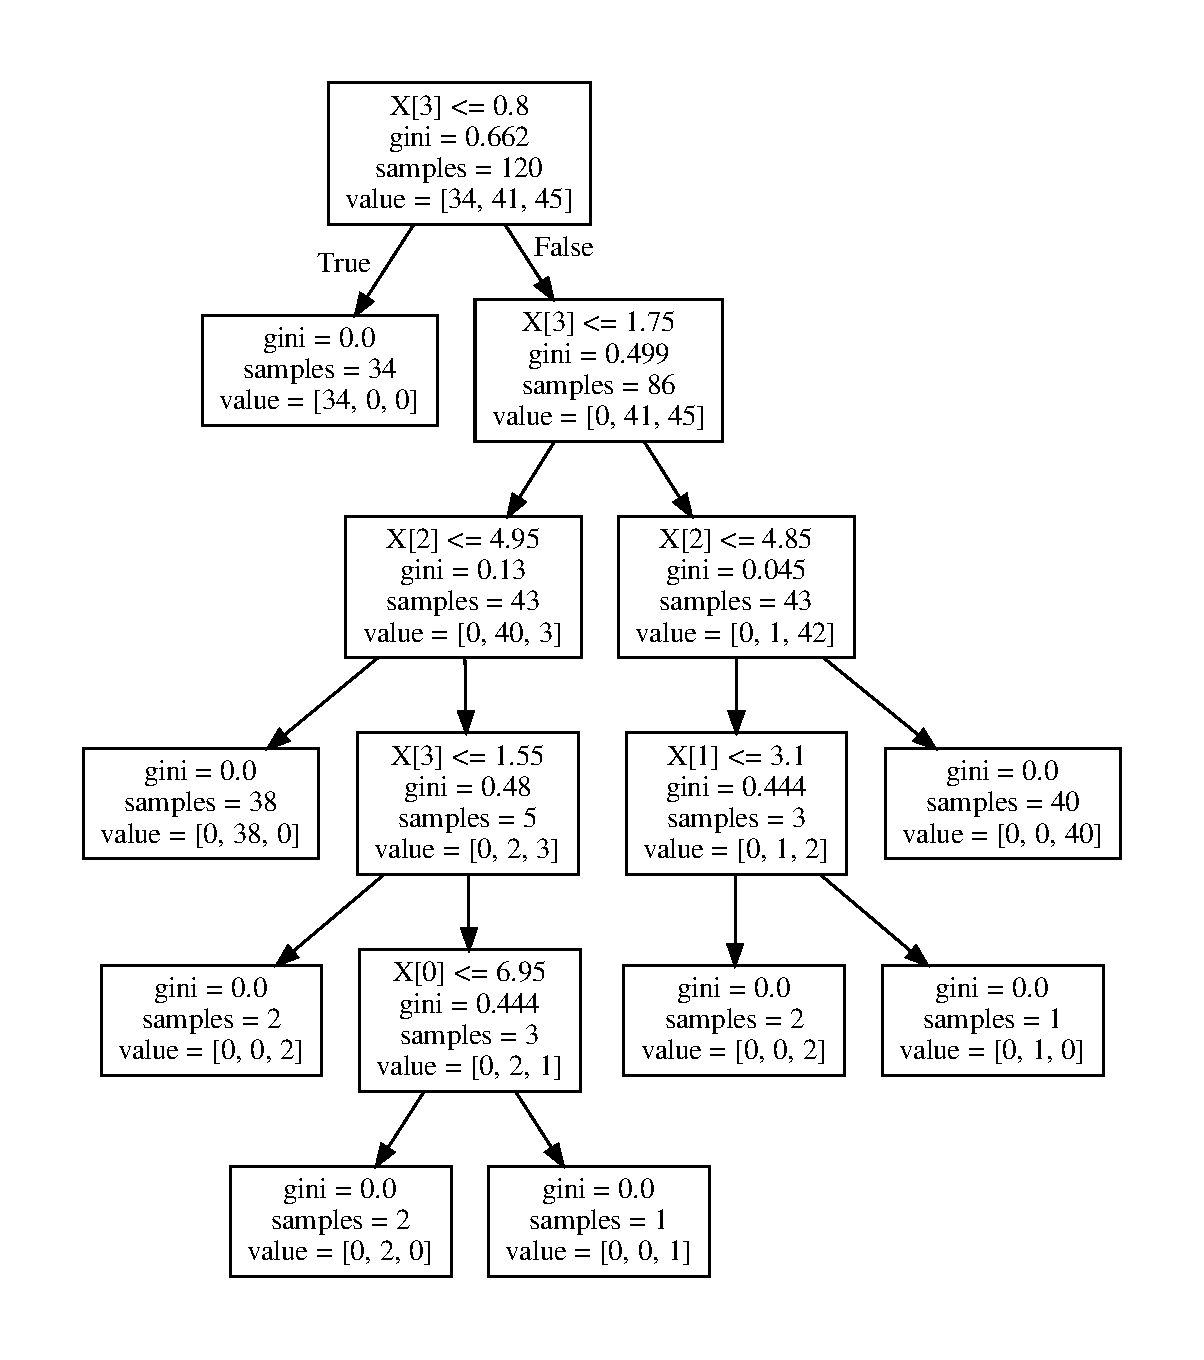
\includegraphics[width=1.0\textwidth]{imgs/decision_tree.pdf}
		\column{0.6\textwidth}
		\begin{itemize}
			\item Creating an if-else conditions automatically
			\item Nested conditions with a parameter to determine how does the separating of the "tree" performs.
		\end{itemize}
	\end{columns}
\end{frame}

\begin{frame}
	\begin{center}
		\begin{figure}
			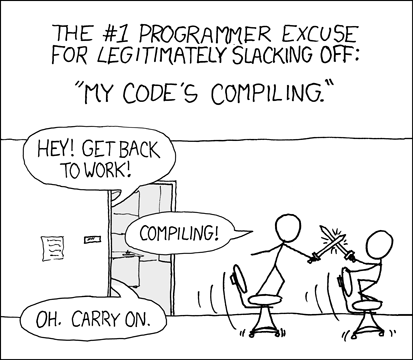
\includegraphics[scale=0.5]{imgs/xkcd_compiling.png}
			\caption{xkcd - Compiling}
		\end{figure}
	\end{center}
\end{frame}

\begin{frame}
	\begin{center}
		\begin{figure}
			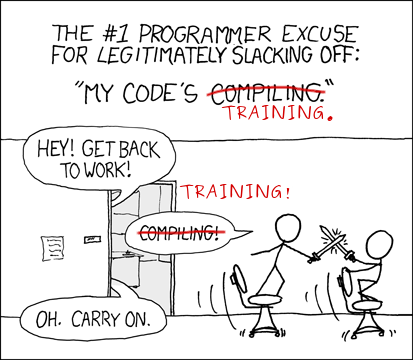
\includegraphics[scale=0.5]{imgs/xkcd_training.png}
			\caption{xkcd - Compiling}
		\end{figure}
	\end{center}
\end{frame}

\section{Problems for Machine Learning}

\subsection{Handwriting recognition}

\begin{frame}
	\frametitle{7-Segment display}
	\begin{columns}
		\column{0.3\textwidth}
		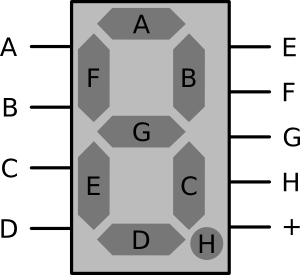
\includegraphics[width=1.0\textwidth]{imgs/7seg.png}
		\column{0.7\textwidth}
		\begin{itemize}
			\item<2-> This is a 7-segment display.
			\item<3-> It consists of a bulb labelled from A-G that could form a number.
		\end{itemize}
		\begin{block}{Problem}<4->
			When the list of the bulb that went on were given, can we determine the number?
		\end{block}
	\end{columns}
\end{frame}

\begin{frame}[fragile]
	\frametitle{7-Segment display}
	\begin{columns}
		\column{0.3\textwidth}
		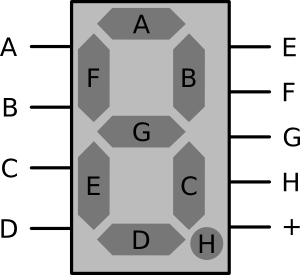
\includegraphics[width=1.0\textwidth]{imgs/7seg.png}
		\column{0.7\textwidth}
		\begin{block}{Problem}
			When the list of the bulb that went on were given, can we determine the number?
		\end{block}
		\onslide<2-> Not only yes, but \textit{easily} yes!
		\begin{lstlisting}<2->
if led_on == (b, c):
    return 1
elif led_on == (a, b, g, e, d):
    return 2
...
\end{lstlisting}
	\end{columns}
\end{frame}

\begin{frame}[fragile]
	\frametitle{Handwriting}
	\begin{columns}
		\column{0.3\textwidth}
		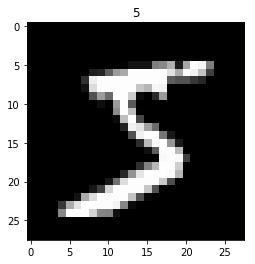
\includegraphics[width=1.0\textwidth]{imgs/mnist_5.png}
		\column{0.7\textwidth}
		\begin{block}{Problem}
			When the image of the handwriting were given, can we determine the number?
		\end{block}
		\onslide<2-> With an \textbf{explicit algorithm}? Obviously no! There are too many ways of drawing the number!
	\end{columns}
\end{frame}

\begin{frame}
	\frametitle{MNIST Dataset}
	\begin{columns}
		\column{0.5\textwidth}
		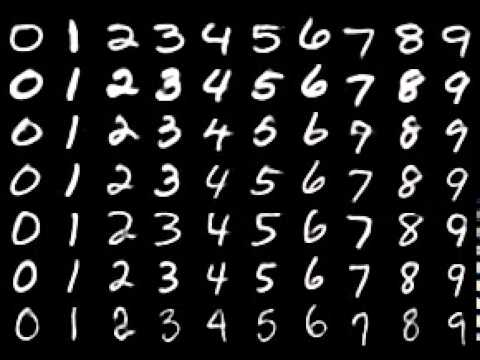
\includegraphics[width=1.0\textwidth]{imgs/mnist.jpeg}
		\column{0.5\textwidth}
		\begin{itemize}
			\item<2-> 28*28 pixel images of handwritten numbers (0-9)
			\begin{itemize}
				\item<3-> Later to be viewed as a vector of 784 dimensions
			\end{itemize}
			\item<4-> 60,000 training images
			\item<5-> 10,000 testing images
		\end{itemize}
	\end{columns}
\end{frame}

\begin{frame}
	\frametitle{$k$-NN with MNIST}
	\begin{itemize}
		\item Training: Pretty fast, no calculations on training phase
		\item Testing: \textit{*thinking*}
			\begin{itemize}
				\item 60,000 data points to calculate the distant + 10,000 data points to test
				\item = 600,000,000 calculations to be made\\
					(this excludes sorting, of which is a $\mathcal{O}(n)$ process)
				\item = \textbf{(relatively) slow}
			\end{itemize}
		\item Good results with $k$-NN were achieved.\\
		($k$-NN w/ non-linear deformation (P2DHMDM), preprocessed with shiftable edges, results into 0.52\% error rate.)
	\end{itemize}
\end{frame}

\begin{frame}
	\frametitle{$k$-NN with MNIST}
	\begin{itemize}
		\item Training: Slow as hell.\\
		{\tiny Trust me, I've tried.}
		\item Good results with SVM were achieved.\\
		(Virtual SVM, deg-9 poly, 2-pixel jittered with deskewing preprocessing results into 0.56\% error rate.)
	\end{itemize}
\end{frame}

\section{Neural Networks}

\begin{frame}
	\frametitle{Artificial Neural Networks (ANN)}
	\begin{columns}
		\column{0.35\textwidth}
		\begin{figure}
			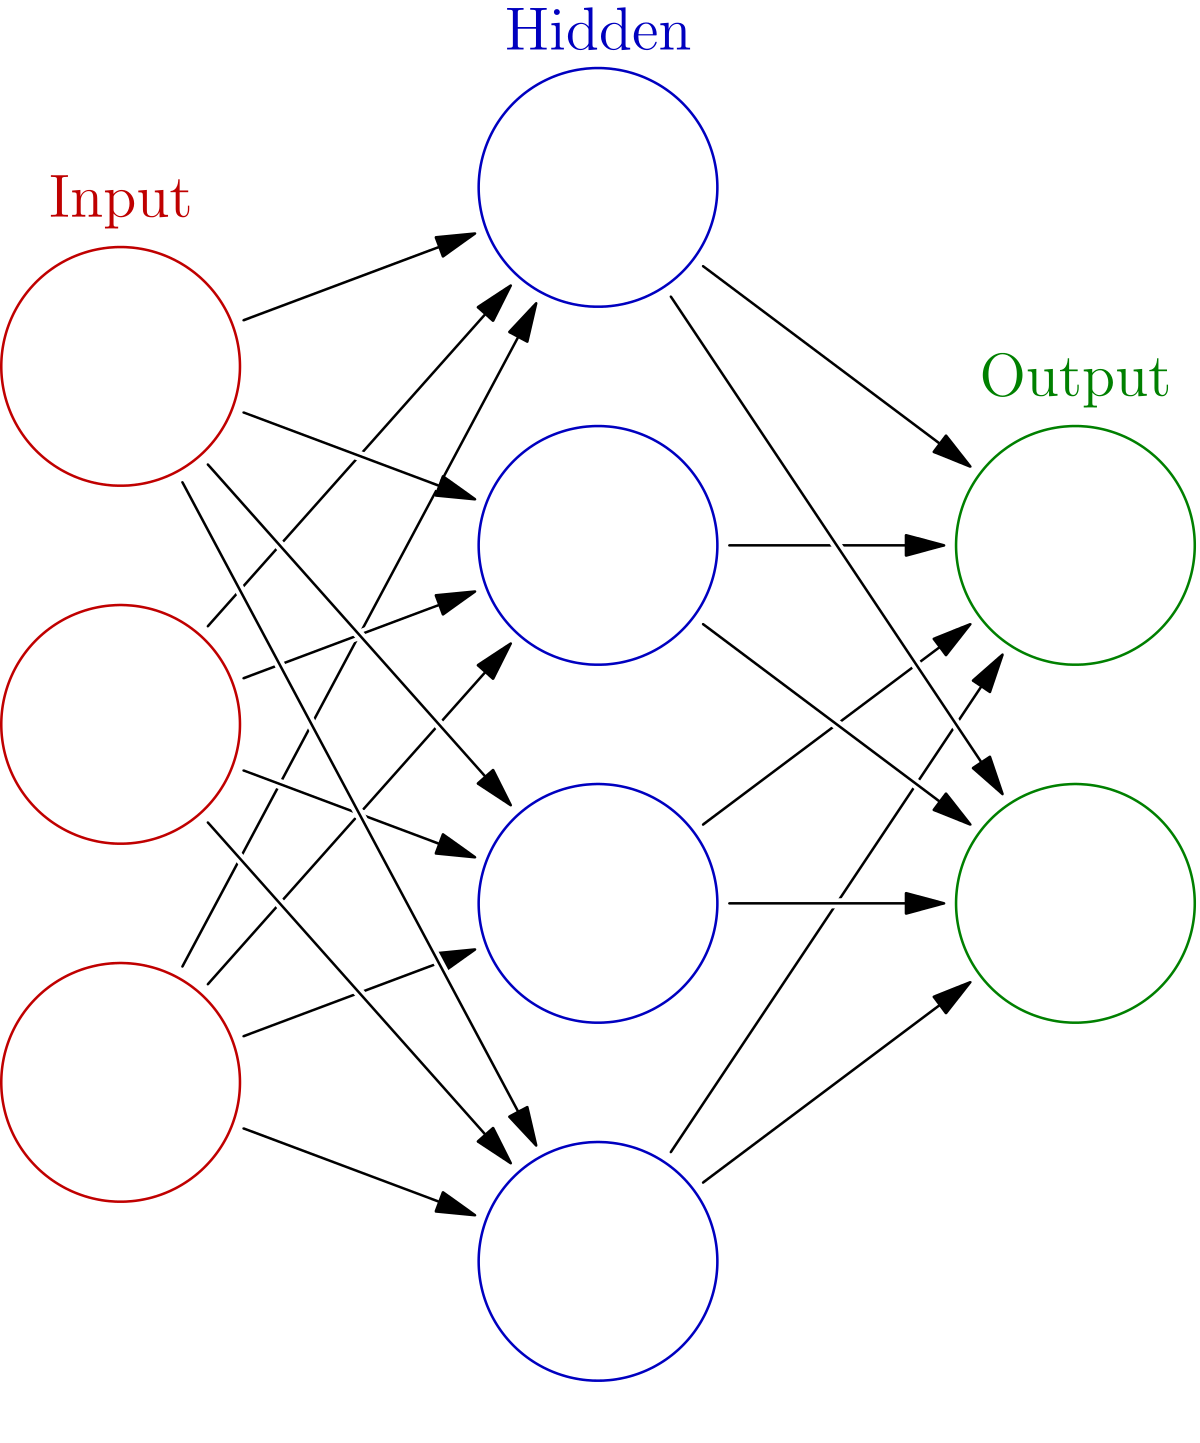
\includegraphics[width=0.8\linewidth,height=0.8\textheight,keepaspectratio]{imgs/ann.png}
			\caption{Neural network (Courtesy: Glosser.ca from Wikimedia Commons)}
		\end{figure}
		\column{0.65\textwidth}
		This seems complex, right? We'll get start a little by little...
	\end{columns}
\end{frame}

\begin{frame}
	\frametitle{Neurons}
	\begin{center}
		\begin{figure}
			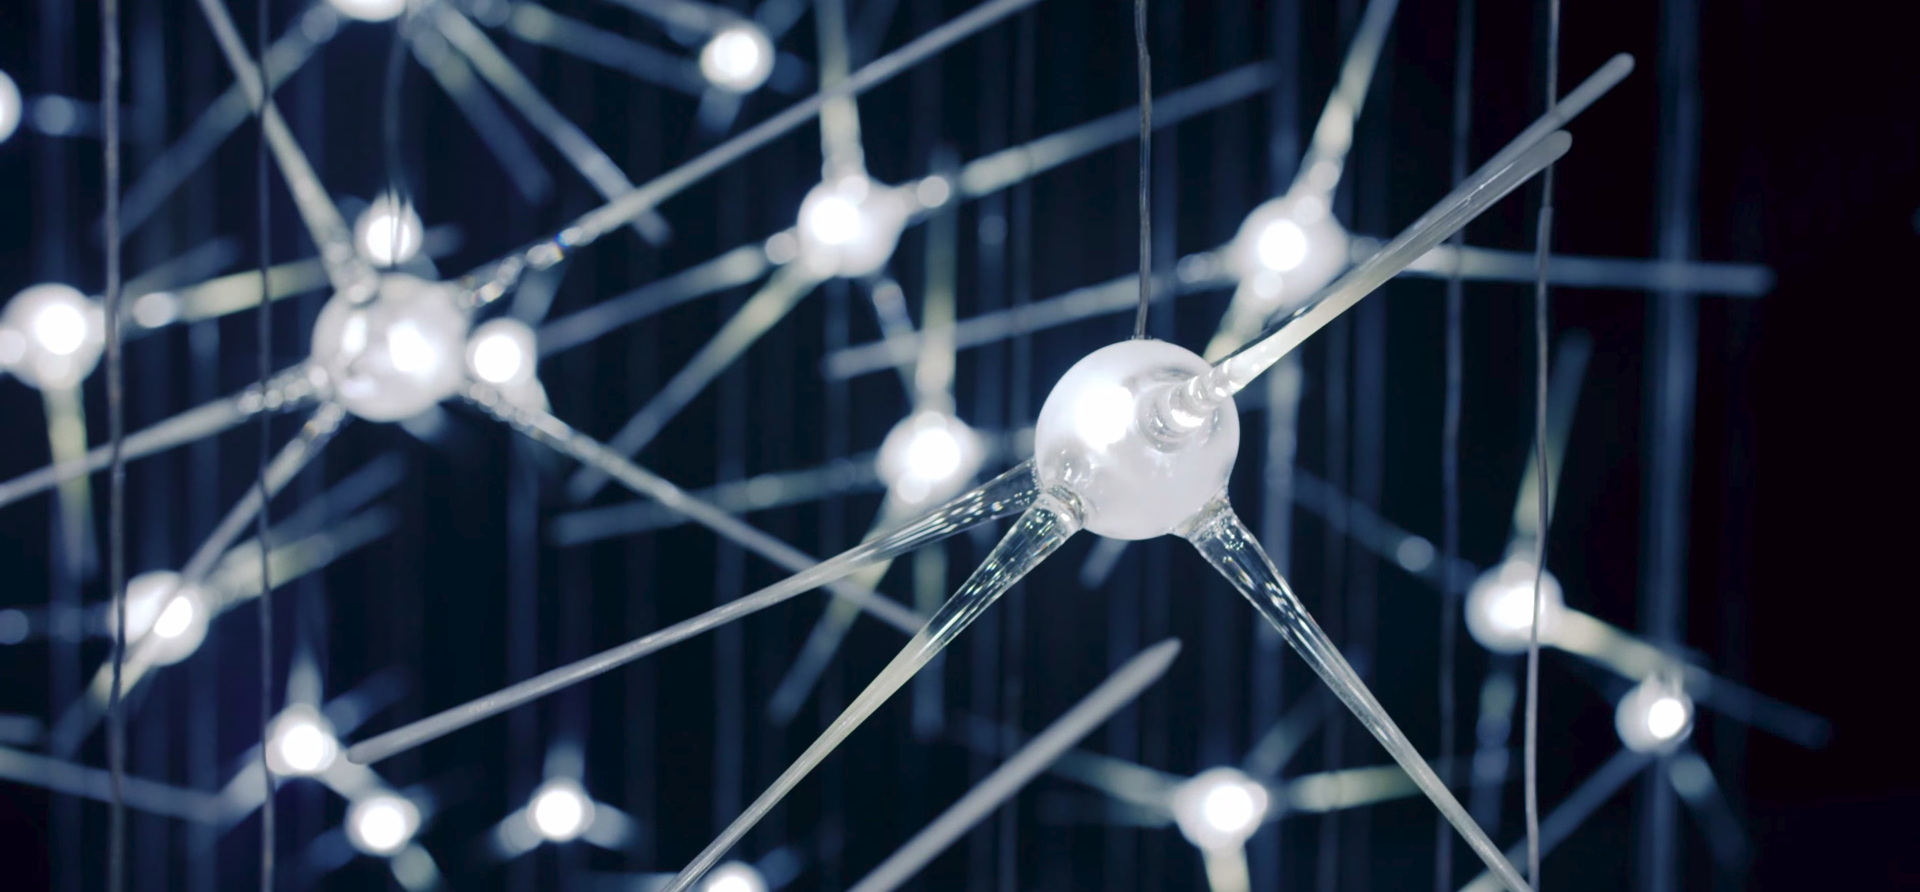
\includegraphics[width=0.8\textwidth]{imgs/neurons_pmh.png}
			\caption{"Neurons" chandelier installed at Princh Mahidol Hall, Nakhon Pathom, Thailand (Courtesy: LASVIT's promotion video)}
		\end{figure}
	\end{center}
\end{frame}

\begin{frame}
	\frametitle{Neuron}
	\begin{center}
		\begin{figure}
			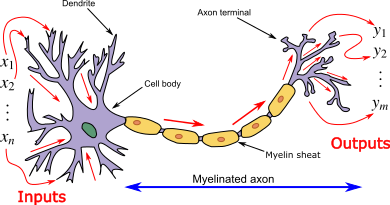
\includegraphics[width=0.7\textwidth]{imgs/neuron.png}
			\caption{Neuron (Courtesy: Egm4313.s12 from Wikimedia Commons)}
		\end{figure}
	\end{center}
\end{frame}

\begin{frame}
	\frametitle{Perceptron}
	\begin{center}
		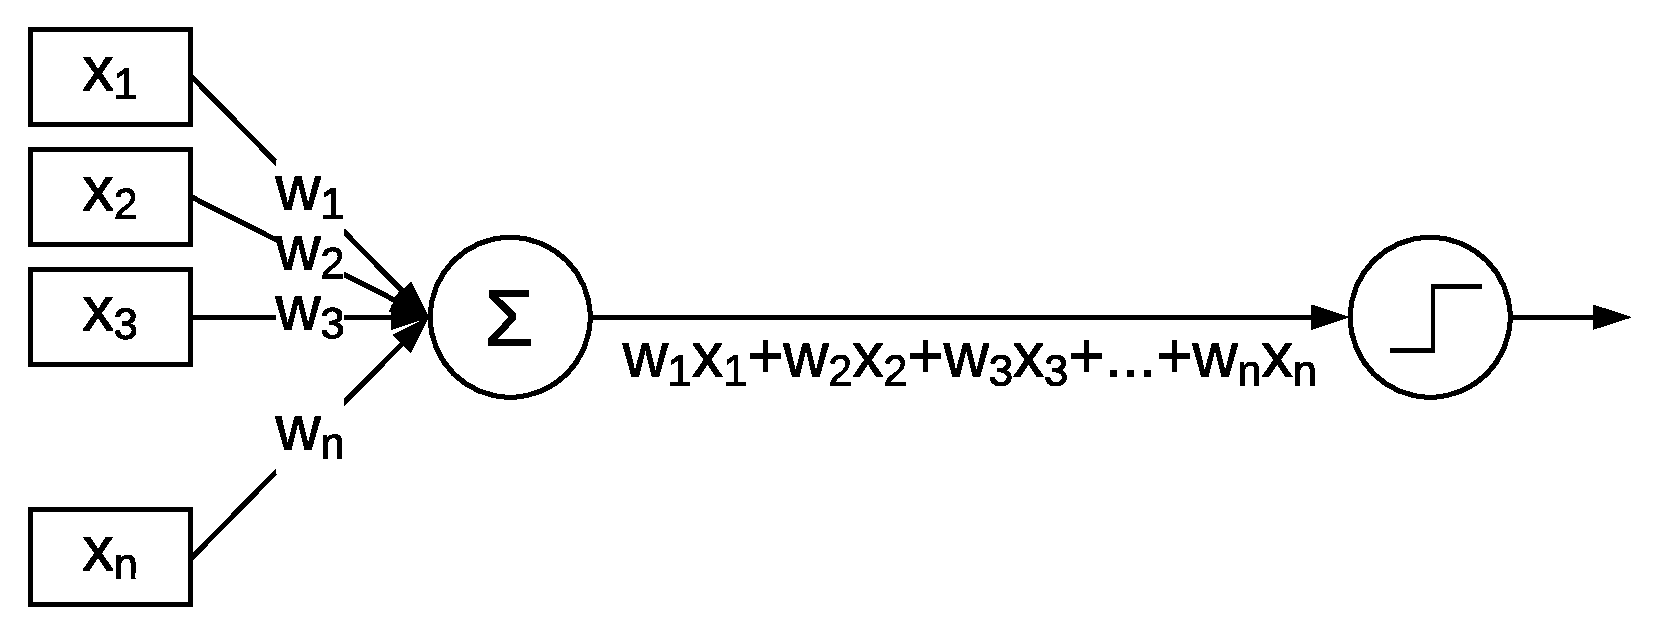
\includegraphics[width=0.7\textwidth]{imgs/perceptron.pdf}
	\end{center}
	\begin{itemize}
		\item \textbf{Inputs} consisting of $n$ inputs from $x_1$, $x_2$ ... to $x_n$.
		\item \textbf{Weights} of each inputs, namely $w_1$, $w_2$, ..., $w_n$
		\item \textbf{Summation} of all the weighted inputs $\Sigma = w_1x_1 + w_2x_2 + \hdots + w_nx_n$
		\item \textbf{Activation function} in either the form of $\Sigma > k$ or  $\Sigma < k (nonlinear)$
	\end{itemize}
\end{frame}

\begin{frame}
	\frametitle{Logic gates with Perceptron}
	\begin{center}
		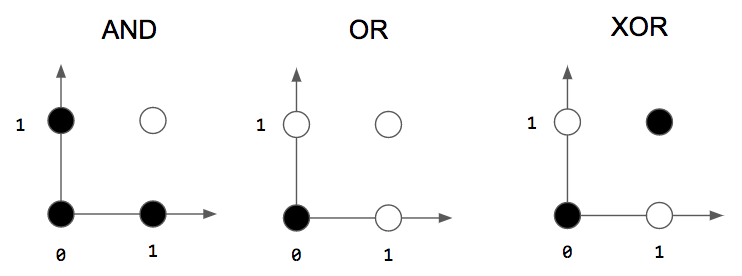
\includegraphics[width=0.7\linewidth,height=0.7\textheight,keepaspectratio]{imgs/gates.png}
	\end{center}
\end{frame}

\begin{frame}
	\frametitle{Logic gates with Perceptron}
	\begin{columns}[t]
		\column{0.33\textwidth}
		{\large AND gate}

		\begin{itemize}
			\item $w_1 = 1$
			\item $w_2 = 1$
			\item $\Sigma = 1x_1 + 1x_2$
			\item $f: \Sigma \geq 2$
		\end{itemize}
		\column{0.33\textwidth}
		{\large OR gate}

		\begin{itemize}
			\item $w_1 = 1$
			\item $w_2 = 1$
			\item $\Sigma = 1x_1 + 1x_2$
			\item $f: \Sigma \geq 1$
		\end{itemize}
		\column{0.33\textwidth}
		{\large XOR gate}

		Why can't XOR gate be created using a perceptron?
	\end{columns}
\end{frame}

\begin{frame}
	\frametitle{Linearly Separable Problem}
	\begin{columns}
		\column{0.4\textwidth}
		\begin{figure}
			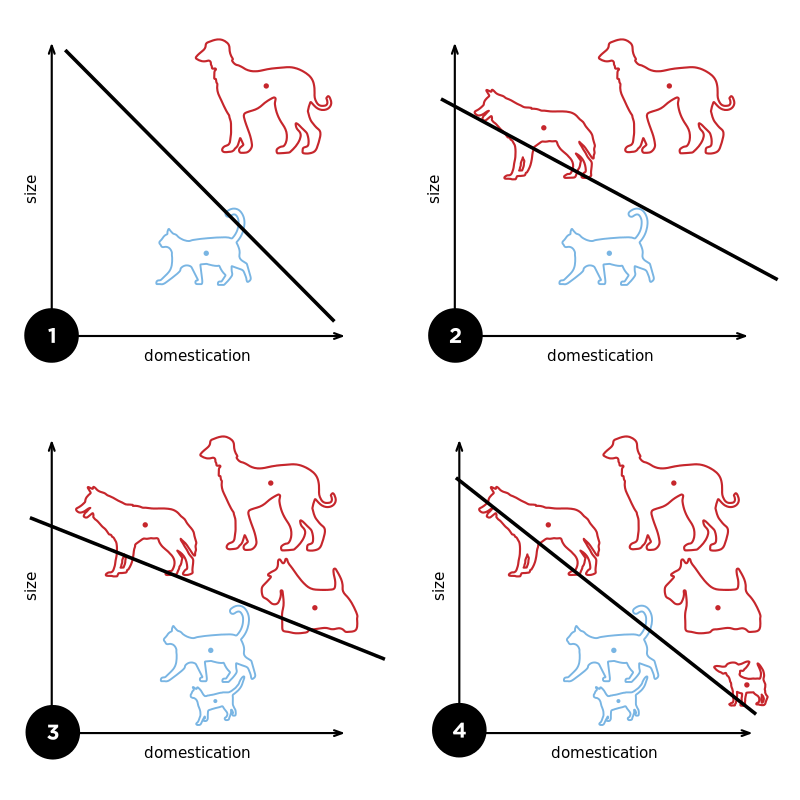
\includegraphics[width=0.7\linewidth,height=0.7\textheight,keepaspectratio]{imgs/linsep.png}
			\caption{Linearly Separable Problem (Courtesy: Elizabeth Goodspeed from Wikimedia Commons)}
		\end{figure}
		\column{0.6\textwidth}
		\begin{itemize}
			\item Now our problem is that the perceptron is a \textbf{linear classifier}, that means it could only separate datas that is linearly separable.
			\item Real-world problems are not that easy to separate
			\item How can we solve this problem?
		\end{itemize}
	\end{columns}
\end{frame}

\begin{frame}
	\frametitle{Artificial Neural Networks}
	\begin{center}
		\begin{figure}
			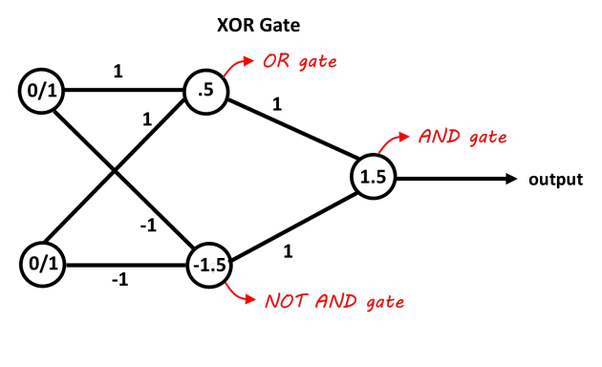
\includegraphics[width=0.7\linewidth,height=0.7\textheight,keepaspectratio]{imgs/xor_nn.png}
			\caption{XOR gate with Perceptrons connected together (Courtesy: Parth Udawant)}
		\end{figure}
	\end{center}
\end{frame}

\begin{frame}
	\frametitle{Artificial Neural Networks}
	How are the weights of each dendrites (inputs) are automatically adjusted?
	\begin{itemize}
		\item<2-> Through a \textbf{backpropagation} Process
		\begin{itemize}
			\item<3-> Initiate weights randomly
			\item<4-> Calculate the error over the training set
			\item<5-> Attempts to adjust weights little by little to minimise loss\\
			{\onslide<6-> \tiny (Seriously, one day it will converge. There exists a mathematical proof)}
		\end{itemize}
	\end{itemize}
\end{frame}

\section{Your next step into Machine Learning}

\begin{frame}
	\frametitle{Courses in KU-CPE to be taken}
	\begin{itemize}
		\item Engineering Mathematics I
		\item Discrete Mathematics and Linear Algebra
		\item Aritificial Intelligence/Machine Learning
	\end{itemize}
\end{frame}

\begin{frame}
	\frametitle{MOOCs}
	For practical use, go ahead with...
	\begin{itemize}
		\item Google's Machine Learning Crash Course
		\item Udemy's Machine Learning (UD120)
	\end{itemize}
\end{frame}

\begin{frame}
	\begin{center}
		{\Huge Thanks!}
		\\~\\
		\url{https://twitter.com/public_srakrn}\\
		\url{https://www.facebook.com/srakrn}\\
		\texttt{sirakorn.l@ku.th}
	\end{center}
\end{frame}
\end{document}